\chapter{Architecture : le réseau qui apprend à débruiter}
\label{chap:architecture}

Les deux chapitres précédents ont défini \emph{ce que} le réseau doit apprendre à prédire
($\varepsilon_\theta$ pour le DDPM, $v_\theta$ pour le flow matching). Ce chapitre décrit \emph{quel}
réseau remplit ce rôle. Un point essentiel structure tout ce chapitre :

\begin{intuition}
Le réseau ignore totalement s'il fait de la diffusion ou du flow matching. Il résout un seul et même
problème de régression : \og étant donné une image $x_t$ dégradée, un temps $t$, et éventuellement un
texte, produis un tenseur de même forme que $x_t$ \fg. Seule l'interprétation de cette sortie (un
bruit ou une vélocité) et la façon dont $x_t$ a été construit diffèrent entre les deux approches. C'est
pourquoi une \textbf{seule et même architecture} — le U-Net décrit ici — est réutilisée sans aucune
modification pour les deux méthodes dans ce projet.
\end{intuition}

\section{Le choix de l'architecture U-Net}

Le réseau doit accomplir une tâche de \emph{traduction image-à-image} : recevoir une image bruitée et
produire une sortie de même résolution spatiale. L'architecture U-Net (Ronneberger et al., 2015,
initialement conçue pour la segmentation d'images médicales) est bien adaptée à ce type de tâche :

\begin{itemize}
    \item une branche \textbf{descendante} (\emph{encoder}) réduit progressivement la résolution
    spatiale tout en augmentant le nombre de canaux, extrayant des caractéristiques de plus en plus
    abstraites ;
    \item une branche \textbf{montante} (\emph{decoder}), symétrique, restaure progressivement la
    résolution d'origine ;
    \item des \textbf{connexions résiduelles} (\emph{skip connections}) relient chaque étage de la
    descente à l'étage de la montée de même résolution, permettant de préserver les détails fins qui
    seraient sinon perdus dans le goulot d'étranglement central.
\end{itemize}

\section{Vue d'ensemble du réseau}

La figure~\ref{fig:unet-architecture} présente l'architecture complète telle qu'implémentée dans ce
projet (configuration par défaut : canaux $[64, 128, 256, 256]$, résolutions $64 \to 32 \to 16 \to 8$).

\begin{figure}[p]
\centering
\resizebox{\textwidth}{!}{% Schéma d'architecture du U-Net partagé (src/backend/shared/unet.py).
% Fidèle à la configuration par défaut : base_channels=64,
% channel_multipliers=(1,2,4,4) -> canaux [64,128,256,256],
% résolutions 64->32->16->8, cross-attention aux étages 32/16/8.
\begin{tikzpicture}[
    font=\small,
    block/.style={draw, rounded corners, minimum width=2.6cm, minimum height=0.85cm, align=center, fill=blue!6},
    attn/.style={draw, rounded corners, minimum width=2.6cm, minimum height=0.65cm, align=center, fill=orange!12},
    io/.style={draw, rounded corners, minimum width=2.6cm, minimum height=0.7cm, align=center, fill=green!8},
    arr/.style={-Stealth, thick},
    skiparr/.style={-Stealth, thick, dashed, gray},
    timearr/.style={-Stealth, thick, purple},
    textarr/.style={-Stealth, thick, orange!80!black},
]

% --- Colonne d'entrée / sortie (gauche) ---
\node[io] (xin) at (0, 0) {$x_t$ \\ $(3,64,64)$};
\node[block] (convin) at (0, -1.4) {Conv$_{3\times3}$ in};

% --- Down path (espacement horizontal augmenté pour laisser respirer les
%     labels downsample/upsample et les flèches d'injection du temps) ---
\node[block] (d0) at (0, -3.0) {ResBlock $\times2$ \\ 64ch, 64$\times$64};
\node[block] (d1) at (3.6, -4.8) {ResBlock $\times2$ \\ 128ch, 32$\times$32};
\node[attn]  (a1) at (3.6, -5.75) {CrossAttn};
\node[block] (d2) at (7.2, -7.2) {ResBlock $\times2$ \\ 256ch, 16$\times$16};
\node[attn]  (a2) at (7.2, -8.15) {CrossAttn};

% --- Bottleneck ---
\node[block] (bn) at (10.8, -9.6) {ResBlock \\ 256ch, 8$\times$8};
\node[attn]  (abn) at (10.8, -10.55) {CrossAttn};
\node[block] (bn2) at (10.8, -11.4) {ResBlock};

% --- Up path (symétrique) ---
\node[block] (u2) at (14.4, -7.2) {ResBlock $\times2$ \\ 256ch, 16$\times$16};
\node[attn]  (au2) at (14.4, -8.15) {CrossAttn};
\node[block] (u1) at (18.0, -4.8) {ResBlock $\times2$ \\ 128ch, 32$\times$32};
\node[attn]  (au1) at (18.0, -5.75) {CrossAttn};
\node[block] (u0) at (21.6, -3.0) {ResBlock $\times2$ \\ 64ch, 64$\times$64};

\node[block] (convout) at (21.6, -1.4) {Conv$_{3\times3}$ out};
\node[io] (xout) at (21.6, 0) {$\varepsilon_\theta$ ou $v_\theta$ \\ $(3,64,64)$};

% --- Flux principal ---
\draw[arr] (xin) -- (convin);
\draw[arr] (convin) -- (d0);
\draw[arr] (d0) -- node[above,sloped,font=\tiny]{downsample} (d1);
\draw[arr] (d1) -- (a1);
\draw[arr] (a1) -- node[above,sloped,font=\tiny]{downsample} (d2);
\draw[arr] (d2) -- (a2);
\draw[arr] (a2) -- node[above,sloped,font=\tiny]{downsample} (bn);
\draw[arr] (bn) -- (abn);
\draw[arr] (abn) -- (bn2);
\draw[arr] (bn2) -- node[above,sloped,font=\tiny]{upsample} (u2);
\draw[arr] (u2) -- (au2);
\draw[arr] (au2) -- node[above,sloped,font=\tiny]{upsample} (u1);
\draw[arr] (u1) -- (au1);
\draw[arr] (au1) -- node[above,sloped,font=\tiny]{upsample} (u0);
\draw[arr] (u0) -- (convout);
\draw[arr] (convout) -- (xout);

% --- Skip connections (concaténation down -> up, même résolution) ---
\draw[skiparr] (d0.east) to[bend left=15] node[above,font=\tiny]{skip} (u0.west);
\draw[skiparr] (a1.east) to[bend left=15] node[above,font=\tiny]{skip} (au1.west);
\draw[skiparr] (a2.east) to[bend left=15] node[above,font=\tiny]{skip} (au2.west);

% --- Injection du temps t : dans CHAQUE ResBlock ---
\node[draw, rounded corners, fill=purple!10, minimum width=2.6cm, minimum height=0.7cm, align=center] (temb) at (10.8, -1.4) {$t \to$ sinusoidal \\ $+$ MLP $\to \vec{t}$};
\foreach \blk in {d0, d1, d2, bn, bn2, u2, u1, u0} {
  \draw[timearr] (temb) -- (\blk);
}

% --- Injection du texte : cross-attention sur chaque bloc d'attention ---
\node[draw, rounded corners, fill=orange!10, minimum width=2.8cm, minimum height=0.7cm, align=center] (text) at (10.8, -13.0) {CLIP texte (gelé) \\ $(77, 512)$};
\foreach \blk in {a1, a2, abn, au2, au1} {
  \draw[textarr] (text) -- (\blk);
}

\end{tikzpicture}
}
\caption{Architecture complète du U-Net partagé. Le flux principal (image) traverse le réseau en
forme de U (traits noirs pleins). Le temps $t$ (violet) est injecté dans \emph{chaque} bloc résiduel,
à toutes les résolutions. Le texte (orange), encodé par CLIP gelé, est injecté par cross-attention aux
résolutions $32\times32$, $16\times16$ et au goulot d'étranglement $8\times8$ — pas à la résolution la
plus fine $64\times64$, où le coût quadratique de l'attention serait trop élevé pour le bénéfice
apporté. Les connexions en pointillés gris sont les skip connections entre étages de même résolution.}
\label{fig:unet-architecture}
\end{figure}

Trois mécanismes assemblent ce réseau ; nous les détaillons dans le reste du chapitre :
\begin{enumerate}
    \item l'\textbf{injection du temps} $t$ (section~\ref{sec:time-embed}), qui indique au réseau à
    quel niveau de dégradation il travaille, à chaque étage ;
    \item le \textbf{bloc résiduel} (\emph{ResBlock}, section~\ref{sec:resblock}), l'unité de base
    répétée à chaque étage ;
    \item l'\textbf{injection du texte} par cross-attention (section~\ref{sec:cross-attn}), qui permet
    au réseau de conditionner sa prédiction sur une description en langage naturel.
\end{enumerate}

\section{Encoder le temps : l'embedding sinusoïdal}
\label{sec:time-embed}

Le réseau reçoit $t$ (un simple entier, ou un flottant continu pour le flow matching) : un scalaire
brut est un signal pauvre et mal exploitable par des couches de convolution. On le transforme d'abord
en un vecteur riche, via un \emph{encodage sinusoïdal} — le même principe que le positional encoding
des Transformers (Vaswani et al., 2017) :
\begin{equation}
    \text{PE}(t, 2i) = \sin\!\left(\frac{t}{10000^{2i/d}}\right), \qquad
    \text{PE}(t, 2i+1) = \cos\!\left(\frac{t}{10000^{2i/d}}\right)
\end{equation}
où $d$ est la dimension de l'encodage et $i \in \{0, \dots, d/2-1\}$ indexe des fréquences
décroissantes. Ce vecteur est ensuite passé dans un petit MLP (\texttt{Linear} $\to$ SiLU $\to$
\texttt{Linear}) pour donner au réseau la capacité d'en tirer une représentation utile à ses propres
besoins internes.

\begin{figure}[h]
\centering
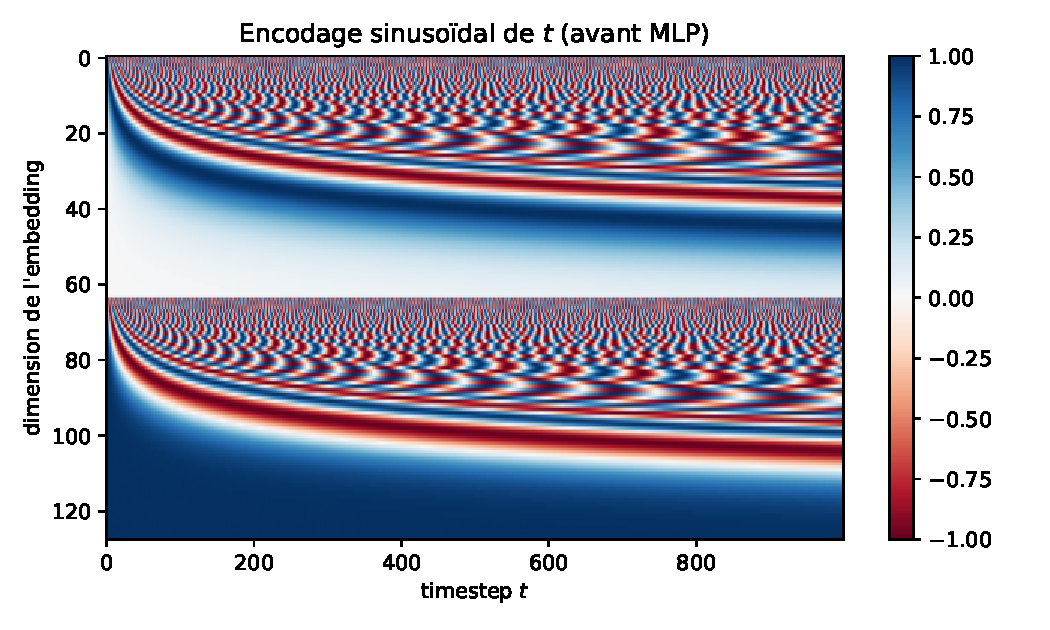
\includegraphics[width=0.75\textwidth]{figures/time_embedding.pdf}
\caption{Visualisation de l'encodage sinusoïdal brut (avant le MLP) pour $d=128$ et $t \in [0, 1000)$.
Chaque ligne horizontale oscille à sa propre fréquence : les dimensions du haut de chaque moitié
(sinus/cosinus) oscillent rapidement (hautes fréquences), celles du bas lentement (basses fréquences).
La combinaison de toutes ces fréquences donne, pour chaque valeur de $t$, une \og signature \fg\ unique
et continue (deux $t$ proches ont des colonnes visuellement proches dans cette figure).}
\label{fig:time-embedding}
\end{figure}

\begin{intuition}
C'est l'analogue d'une horloge à plusieurs aiguilles tournant à des vitesses différentes (secondes,
minutes, heures) : en lisant la position de toutes les aiguilles simultanément, on identifie un instant
précis. Ici, chaque dimension de l'embedding est une \og aiguille \fg\ tournant à sa fréquence propre en
fonction de $t$.
\end{intuition}

Le vecteur final, noté $\vec t \in \mathbb{R}^{d_{\text{temps}}}$ (dimension $512$ dans ce projet),
n'est \textbf{pas} donné une seule fois en entrée du réseau : il est ré-injecté dans \emph{chaque}
ResBlock, à \emph{chaque} étage de résolution (flèches violettes de la figure~\ref{fig:unet-architecture}).

\section{Le bloc résiduel (ResBlock)}
\label{sec:resblock}

C'est l'unité de calcul de base, répétée à chaque étage du U-Net. Son rôle est double : extraire des
caractéristiques locales de l'image par convolution, et moduler ce calcul en fonction du temps $\vec t$.

\begin{equation}
\begin{aligned}
    h &= \text{Conv}_{3\times3}\big(\text{SiLU}(\text{GroupNorm}(x))\big) \\
    h &= h + \text{Linear}(\vec t)_{\ \text{broadcast sur } H,W} \\
    h &= \text{Conv}_{3\times3}\big(\text{SiLU}(\text{GroupNorm}(h))\big) \\
    \text{sortie} &= h + \text{skip}(x)
\end{aligned}
\end{equation}

où $\text{skip}(x) = x$ si le nombre de canaux ne change pas, et $\text{skip}(x) = \text{Conv}_{1\times1}(x)$
sinon (pour ajuster la dimension avant l'addition résiduelle).

\begin{intuition}
La projection linéaire de $\vec t$, additionnée aux feature maps après la première convolution, agit
comme un \og biais dépendant du contexte \fg : elle décale toutes les activations d'une quantité qui
dépend du niveau de bruit courant, permettant au même jeu de poids de convolution de se comporter
différemment selon que l'on débruite une image très bruitée ($t$ grand) ou presque propre ($t$ petit).
\end{intuition}

La connexion résiduelle ($h + \text{skip}(x)$) suit le principe des ResNets (He et al., 2015) : elle
facilite la propagation du gradient à travers un réseau profond (rappelons que le U-Net complet
comporte des dizaines de ces blocs empilés), en donnant au réseau la possibilité d'apprendre une
simple perturbation de l'entrée plutôt qu'une transformation complète.

\section{Conditionner sur le texte : la cross-attention}
\label{sec:cross-attn}

\subsection{Représenter le texte : CLIP}
\label{sec:clip}

Comprendre du texte libre (grammaire, synonymes, combinaisons d'attributs) demande d'avoir vu une
quantité de langage bien supérieure à ce qu'un jeu de données de quelques centaines de milliers de
légendes peut fournir à un encodeur entraîné \emph{from scratch}. Ce projet réutilise donc un encodeur
de texte \textbf{pré-entraîné et gelé} : le \emph{text encoder} de CLIP (Radford et al., 2021)
\cite{radford2021clip}, dont les poids ne sont \textbf{jamais mis à jour} pendant l'entraînement —
seul le U-Net apprend.

CLIP a été entraîné à aligner des représentations de texte et d'image sur des centaines de millions de
paires (image, légende) : ses embeddings capturent donc déjà des notions visuelles pertinentes
(\og souriant \fg, \og lunettes \fg\ sont représentés de façon cohérente avec leur contenu visuel),
même si CLIP lui-même n'a jamais vu le jeu de données CelebA-Dialog. Une phrase en entrée produit une
séquence d'embeddings, un par token :
\begin{equation}
    \text{texte} \xrightarrow{\ \text{CLIP (gelé)}\ } \text{embed} \in \mathbb{R}^{77 \times 512}
\end{equation}
(77 étant la longueur de séquence maximale standard de CLIP, avec padding pour les phrases plus courtes).

\subsection{Le mécanisme de cross-attention}

Une fois le texte encodé, comment le U-Net l'utilise-t-il ? La réponse est l'\textbf{attention croisée}
(\emph{cross-attention}), le même mécanisme central des Transformers (Vaswani et al., 2017), mais
appliqué entre deux modalités différentes (image et texte) plutôt qu'au sein d'une seule séquence.

\begin{figure}[h]
\centering
\resizebox{0.85\textwidth}{!}{% Schéma du mécanisme de cross-attention texte -> image (src/backend/shared/unet_blocks.py, CrossAttentionBlock).
\begin{tikzpicture}[
    font=\small,
    block/.style={draw, rounded corners, minimum width=2.4cm, minimum height=0.8cm, align=center},
    arr/.style={-Stealth, thick},
]

\node[block, fill=blue!8] (img) at (0, 3) {feature map image \\ $(B, C, H, W)$};
\node[block, fill=blue!8] (flat) at (0, 1.6) {aplatie en séquence \\ $(B, HW, C)$};
\node[block, fill=blue!15] (q) at (0, 0.2) {$Q = W_Q \cdot h$ \\ $(B, HW, C)$};

\node[block, fill=orange!8] (txt) at (7, 3) {embeddings CLIP \\ $(B, 77, 512)$};
\node[block, fill=orange!15] (k) at (5.5, 1.6) {$K = W_K \cdot \text{texte}$};
\node[block, fill=orange!15] (v) at (8.5, 1.6) {$V = W_V \cdot \text{texte}$};

\node[block, fill=green!12, minimum width=5cm] (attn) at (3.5, -1.4) {$\text{Attention}(Q,K,V) = \text{softmax}\!\left(\dfrac{QK^\top}{\sqrt{d}}\right) V$};

\node[block, fill=blue!8] (out) at (3.5, -3) {$+$ résiduel, reshape \\ $(B, C, H, W)$};

\draw[arr] (img) -- (flat);
\draw[arr] (flat) -- (q);
\draw[arr] (txt) -- (k);
\draw[arr] (txt) -- (v);
\draw[arr] (q) -- (attn);
\draw[arr] (k) -- (attn);
\draw[arr] (v) -- (attn);
\draw[arr] (attn) -- (out);
\draw[arr, dashed, gray] (img.south) to[bend right=35] node[left, font=\tiny]{skip} (out.west);

\end{tikzpicture}
}
\caption{Mécanisme de cross-attention texte $\to$ image utilisé dans chaque bloc \texttt{CrossAttentionBlock}
du U-Net. Les positions spatiales de la feature map image forment les requêtes (\emph{queries}) ; les
tokens du texte fournissent les clés (\emph{keys}) et valeurs (\emph{values}).}
\label{fig:cross-attention}
\end{figure}

Concrètement, à une résolution donnée, la feature map image de forme $(B, C, H, W)$ est aplatie en une
séquence de $H \times W$ \og pixels \fg, chacun projeté en une requête $Q$. Le texte fournit les clés
$K$ et valeurs $V$. L'attention standard est alors calculée :
\begin{equation}
    \text{Attention}(Q, K, V) = \text{softmax}\!\left(\frac{QK^\top}{\sqrt{d}}\right) V
\end{equation}

\begin{intuition}
Chaque position spatiale de l'image \og interroge \fg\ tous les mots de la phrase et récupère une
combinaison pondérée de l'information qu'ils encodent, pondérée par leur pertinence pour cette
position précise. Par exemple, les positions spatiales correspondant à la zone de la bouche
apprendront, au fil de l'entraînement, à accorder plus de poids aux tokens liés au sourire si la
légende en mentionne un.
\end{intuition}

Comme pour le ResBlock, une connexion résiduelle est appliquée : la sortie de l'attention est
\textbf{ajoutée} à la feature map d'entrée plutôt que de la remplacer, ce qui permet au réseau
d'apprendre progressivement à quel point utiliser l'information textuelle à cet endroit précis du
réseau.

\subsection{Où placer les blocs de cross-attention ?}

Le coût de calcul de l'attention standard est quadratique en le nombre de positions
($O((HW)^2)$) : l'appliquer à la résolution la plus fine ($64\times64 = 4096$ positions) serait
prohibitif. Ce projet suit le choix standard (repris de Stable Diffusion) d'activer la cross-attention
uniquement aux résolutions intermédiaires et basses ($32\times32$, $16\times16$, et le goulot
d'étranglement $8\times8$), où le nombre de positions reste raisonnable tout en donnant au réseau
suffisamment d'occasions d'intégrer l'information textuelle à différentes échelles de représentation.
